%!TEX root = ../thesis.tex

\thispagestyle{myheadings}

\graphicspath{{Body/Figures/WaGeneral/Temporary/}{Body/Figures/WaGeneral/Reconstruction/}{Body/Figures/WaGeneral/Histogramming/}{Body/Figures/WaGeneral/Pileup/}{Body/Figures/WaGeneral/Pileup/TimeAndEnergySpectra/}{Body/Figures/RatioAnalysis/}{Body/Figures/RatioAnalysis/MethodOverview/}}

\chapter{\texorpdfstring{\wa}{wa} Measurement}
\label{chapter:wa}


The measurement of \wa is determined by counting the number of detected positrons in the calorimeters above some energy threshold, as described in \secref{section:WaIntro}. Doing so results in a histogram of counts which is modulated by \wa, \figref{fig:gm2wiggle}. Fitting for the frequency allows \wa to be extracted. The \wa measurement therefore consists of the steps needed to construct the histogram of counts, the fitting of that histogram, and any systematic studies done in the analysis. 


\section{Reconstruction of decay positron hits}
\label{sec:ReconWest}


The calorimeters measure hit times and energies of impacting particles, where these hit times and energies are determined from the raw SiPM signals and a reconstruction procedure. In E989 there are two overall separate reconstruction algorithms, \texttt{ReconWest} and \texttt{ReconEast}, both written in the \textit{art} framework similar to the tracking reconstruction. Each of these reconstruction algorithms is modularized, and the steps of the reconstruction process can be switched in and out at will. Using separate reconstruction methods gives confidence in any final results by removing single points of failure. The reconstruction method used in this analysis is \texttt{ReconWest}. A summary of its details will be presented here. A more thorough description is detailed by A. Fienberg \cite{AFThesis}.


The raw data are digitized waveforms, which are voltage versus time traces output from each SiPM for each calorimeter crystal hit. Due to the incredible amount of data coming in with the high muon fill rate, only those pulses which exceed some threshold are saved to disk. An online processing system checks the traces against this pre-configured threshold by passing all of the data through a GPU farm \cite{Gohn:2016shi}. If any trace is found above threshold, then the data is saved from every SiPM in every calorimeter, for a time range around the over-threshold trace. This time range is called a time island, similar to that in the tracking reconstruction, and typically has a width of $\SI{40}{ns}$ \cite{AFThesis}.


The traces are then fit with templates in order to extract the the area and peak times of any present pulses. Each SiPM has its own templates, one for positrons and one for laser pulses. These templates are extracted from data, where each template is determined by collecting many single pulse traces from a SiPM, normalizing by pulse area, aligning in time, and averaging them. These templates were checked against many systematic effects in order to make sure that the constructed templates did not bias the energy or time measurements, such as hit angle, energy (pulse size), position, and rate, as well as aging effects \cite{Kaspar:2016ofv,AFThesis}. Each trace is fit using a \chisq minimization algorithm with the corresponding SiPM templates in order to determine the time and energy of the hit. In order to fit for multiple pulses in a single time island, the fitting procedure first fits with a single template, and then checks the residuals for any remaining peaks. If peaks exist above some threshold, then the fitting is repeated until all pulses have been fit. The time measurement performance in the pulse finding was found to be unaffected by the number of pulses in a time island, and there is 100\% pileup separation at \ns{5} \cite{AFThesis}. See \figref{fig:TemplateFit} for a typical single template fit to a SiPM trace.


\begin{figure}[]
    \centering
    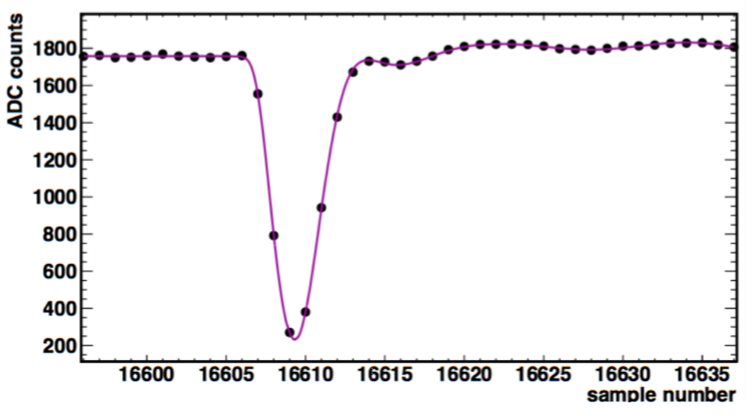
\includegraphics[width=0.6\textwidth]{TemplateFit}
    \caption[Template fit to SiPM trace]{A template fit in purple to a SiPM trace delineated by the black points which is in units of ADC counts. Plot courtesy of Aaron Fienberg.}
    \label{fig:TemplateFit}
\end{figure}


Once a pulse has been fit with a template, the pulse area needs to be converted to real energy units using an energy calibration procedure. A couple of different techniques exist that can be used, including a method that counts photo-statistics seen in the SiPMs \cite{AFThesis}. The default method used is a comparison of lost muon energy signatures in the calorimeters. As described in \refref{lostmuons}, muons lost from the storage ring can spiral inward and hit consecutive calorimeters with a specific time separation between calorimeter hits. These lost muons are minimum-ionizing particles, and thus leave a very distinct energy signature in the crystals, see \secref{sec:lostmuons}. Selecting on the time signature allows hits corresponding to lost muons to be isolated, and the energy signature can be used to determine the appropriate conversions from area to energy\footnote{Different channels can also be equalized based on the energy signatures.}. 


The energy calibration for positron hits as compared to lost muon hits then needs to be determined. Again there are a couple of different techniques, including a comparison of endpoint energies for high energy positrons which tail off at the magic momentum of $\SI{3.094}{\GeV}$, and comparison with simulation. The default technique is to calibrate the energies such that the optimal energy threshold for the \wa analysis is near $\SI{1.7}{\GeV}$ \cite{AFThesis}. Ultimately the energy calibration doesn't matter too much because it is not the energy units that really matter. What really matters is the number of positrons above some energy threshold, where that threshold can be optimized empirically. In fact, the entire \wa analysis could be done without even considering the energy of the incident positrons, and only considering the area of the SiPM pulses\footnote{This statement ignores the effects of pileup which must be accounted for, and applies for a threshold style analysis, and not for other analysis methods which depend on the energy of the pulses.}.


Each pulse fit now has an associated energy and time. Because the measurement of \wa depends heavily on the time reconstruction since the analysis is a frequency extraction, pulse times need to be corrected for various effects in order to reach the precision goal. The fitted times for each pulse need to be aligned on a fill-by-fill basis relative to the injection time of the beam, corrected for any channel differences due to differing pulse shapes or fiber lengths, and corrected for any calorimeter time misalignments due to the use of different laser system components. The fill-by-fill alignment is corrected for using the T0 detector as described in \secref{sec:T0}. The channel differences are corrected by aligning calorimeter channels in time using signals from islands with large simultaneous pulses in neighboring crystals. Calorimeters are time aligned using lost muon coincident events as described before. Once the times of the pulse fits or crystal hits have been determined, the energies can be corrected appropriately for gain effects measured by the laser system. As described in \secref{sub:LaserCalibrationSystem}, the laser calibration system corrects for in-fill, out-of-fill, and SDTP effects \cite{Gain}. \figref{fig:IFGFunction} shows an in-fill gain function fit to data for a single calorimeter. Systematic effects for corrected gain effects are studied in \secref{sub:gainerror}. 

\begin{figure}[]
    \centering
    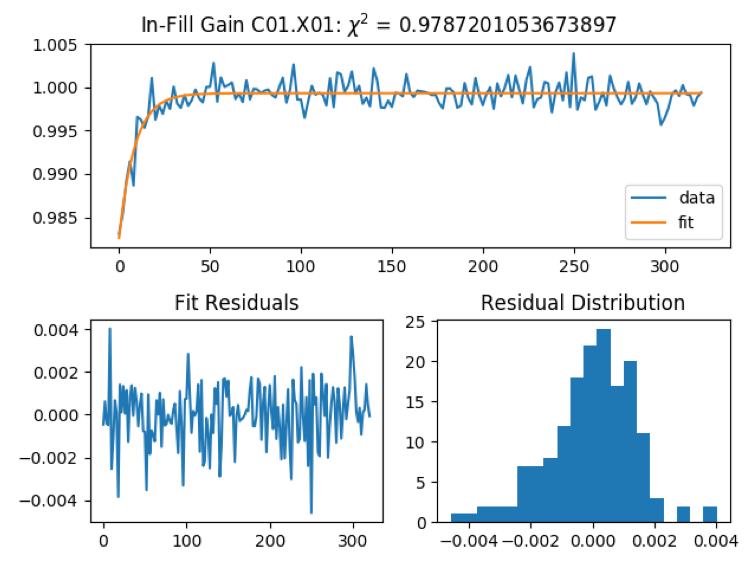
\includegraphics[width=0.6\textwidth]{IFGFunction}
    \caption[In-fill gain function fit for a single calorimeter crystal]{In-fill gain function fit for a single calorimeter crystal (top) and fit residuals (bottom). Each crystal has its own in-fill and SDTP gain function parameters. Plot courtesy of Matthias Smith.}
    \label{fig:IFGFunction}
\end{figure}


The last part of the calorimeter reconstruction is the clustering. Clustering is the stage which takes the individual template fit results from separate crystals, and turns them into the times, energies, and positions of decay positron impacts. For a time island with a single positron impact, the procedure is straightforward. The energy for the positron hit cluster is the sum of the individual hit crystal energies. The time for the cluster is taken as the time of the maximum energy hit in the island. This works because most of the deposited energy from a hit is localized to a single crystal. The position of the cluster is determined with a logarithmic weighting function between crystal hits, which for a $\SI{2}{\GeV}$ positron in the E989 calorimeters results in a resolution of $\SI{2}{mm}$ \cite{AFThesis}. See \figref{fig:CaloCluster} for a single calorimeter cluster from a positron hit in the calorimeter. For a time island with multiple positron impacts, the individual crystal hits are separated in time, where the time partitioning separates hits that are $\SI{2.5}{ns}$ apart, and the clustering proceeds as before. For hits which are within this time window, a pileup event has occurred. If the pileup event happens within the same crystal, then the multiple hits are measured as a single hit, and this needs to be corrected for using a pileup subtraction technique, as described in \secref{sub:pileupsubtraction}. For hits that occur in separate crystals, the pileup can be resolved using the spatial separation of the calorimeters. This is an ongoing area of work, and one technique is described in \refref{AFThesis}. For this analysis the spatial separation was turned off, which simplifies the analysis somewhat. This increases the amount of pileup seen in the data, which then needs to be handled by the pileup subtraction technique. For the precision of the Run 1 analysis result, this was found to be acceptable. 


\begin{figure}[]
    \centering
    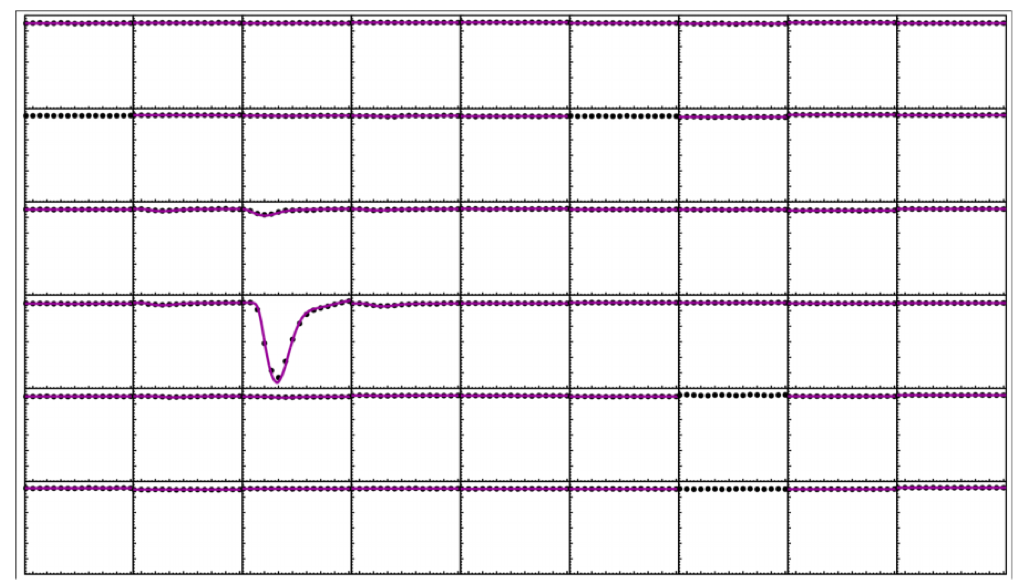
\includegraphics[width=0.9\textwidth]{CaloCluster}
    \caption[Calorimeter cluster from SiPM traces fit with templates]{A single positron hit in the calorimeter, which resulted in a reconstructed calorimeter cluster. Each box is a crystal in the calorimeter, where the contained trace is the SiPM output fit with a template. The positron hit the crystal three from the left and three from the bottom, where it deposited most of its energy. Some of the energy was deposited in the neighboring crystals. Plot courtesy of Aaron Fienberg.}
    \label{fig:CaloCluster}
\end{figure}



\section{Construction of hit energy and time spectra}
\label{sec:Histogramming}


Once the reconstruction has processed all calorimeter hits into clusters, the energy and time spectra histograms are made. At the very last stage of the reconstruction procedure, an \textit{art} module takes the produced clusters and puts them into \ROOT \texttt{TTree} formats, where individual data members include the energies, times, calorimeter numbers, etc. of the individual clusters. There is of order 20,000--140,000 cluster data files per dataset, which are combined down to order 200--1,400 \ROOT \texttt{TTree} files. These \ROOT \texttt{TTree}s are then passed through a \ROOT macro to produce \ROOT files with the histograms defined by the \texttt{TH1F} class, one \ROOT histogram file per tree file.


It should be noted that some of the parameter choices for the constructed histograms were informed by analysis results. All analysis parameters were chosen to be identical between the distinct analyzed datasets, in order to simplify both the comparison and combination of different dataset results. This section describes the justification for the different histogram parameters chosen. A table of the histogram parameters is shown in \tabref{tab:histogramparameters}.


\begin{table}[]
\centering
\setlength\tabcolsep{10pt}
\renewcommand{\arraystretch}{1.2}
\begin{tabular*}{.8\linewidth}{@{\extracolsep{\fill}}lc}
  \hline
    \multicolumn{2}{c}{\textbf{Time Spectra Parameters}} \\
  \hline\hline
    Parameter & Value \\
  \hline
    Energy threshold $(E_{th})$ & $\SI{1700}{\MeV}$ \\
    Bin width $(T_{c})$ & $\SI{149.2}{ns}$ \\
    Artifical dead time (ADT) & $\SI{6}{ns}$ \\
    Shadow dead time (SDT) & $\SI{6}{ns}$ \\
    Shadow gap time (SGT) & $\SI{12}{ns}$ \\
    Pileup energy scaling (C) & $1$ \\
    \gmtwo period $(T_{a})$ in Ratio Method & \mus{4.365411} \\
    Muon lifetime (\taumu) in Ratio Method & \mus{64.44} \\
  \hline 
\end{tabular*}
\caption[Parameters used in the construction of \wa time spectra]{Parameters used in the construction of \wa time spectra. \textbf{fill this table out more once I've gone through the various parts}}
\label{tab:histogramparameters}
\end{table}


Energy and time histograms are made for each individual calorimeter. These are summed together to form histograms of all hit times and energies. An energy threshold is applied to the clusters before filling the time histograms. As described at the end of \secref{section:WaIntro}, the optimal energy threshold is where the quantity $NA^{2}$ reaches the maximum, at least in the case of a five parameter fit\footnote{Using the final fit function and looking at the error directly on the fitted \wa frequency, a slightly better estimate can be found.}. By scanning over the choice of energy threshold and fitting the resulting time spectra with \equref{eq:5parfunc}, the optimal energy threshold can be determined as seen in \figref{fig:OptimalEnergyThreshold}. The optimal choice of energy threshold was determined to be $\SI{1700}{\MeV}$, in accordance with the cluster reconstruction energy calibration. 

    \begin{figure}[]
    \centering
        \begin{subfigure}[t]{0.45\textwidth}
            \centering
            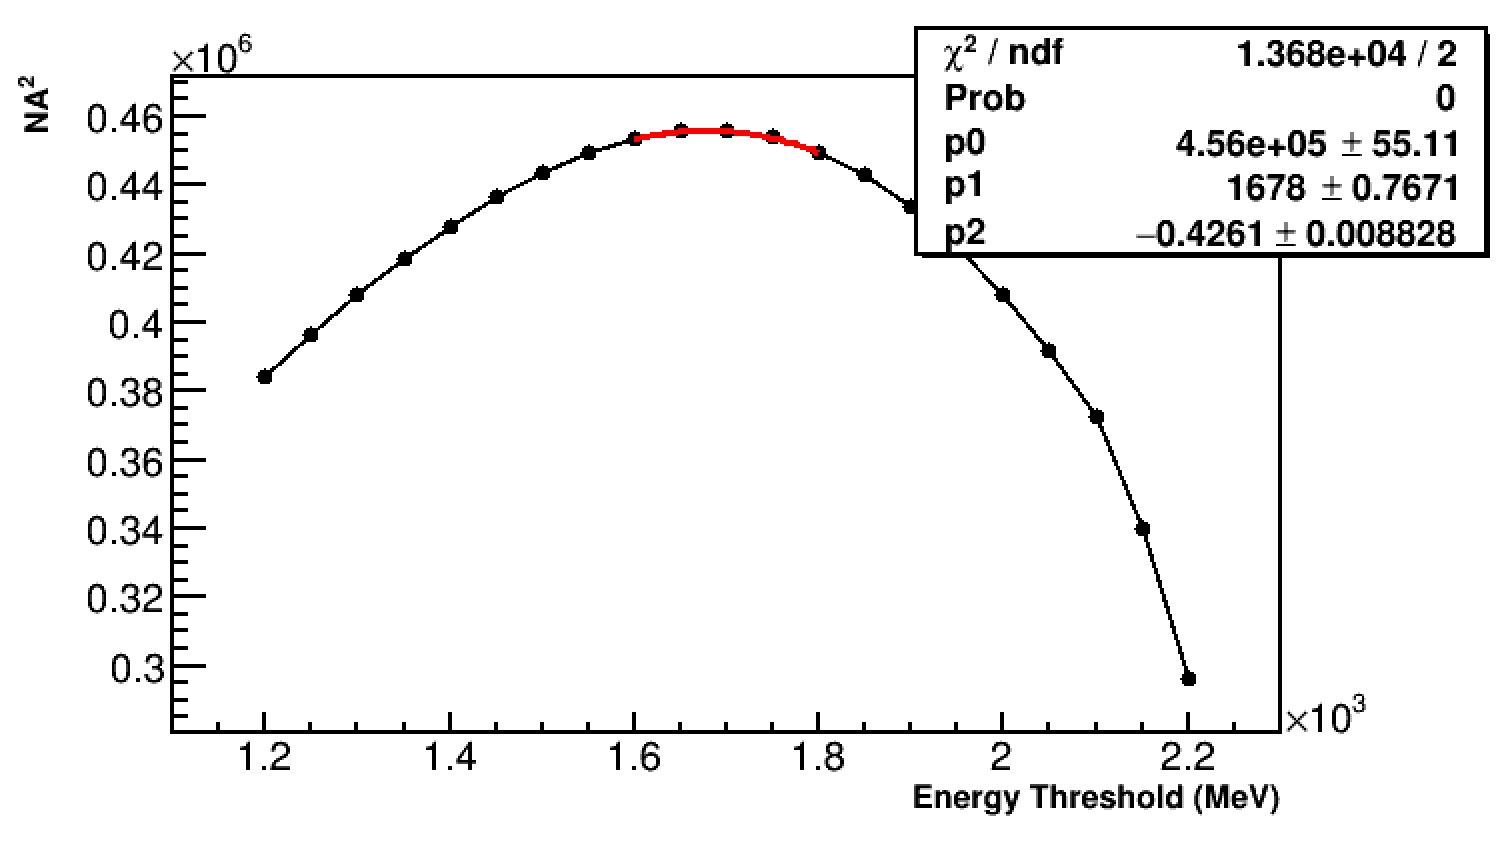
\includegraphics[width=\textwidth]{TemporaryEThresholdNA2}
            \caption{}
        \end{subfigure}
        \begin{subfigure}[t]{0.45\textwidth}
            \centering
            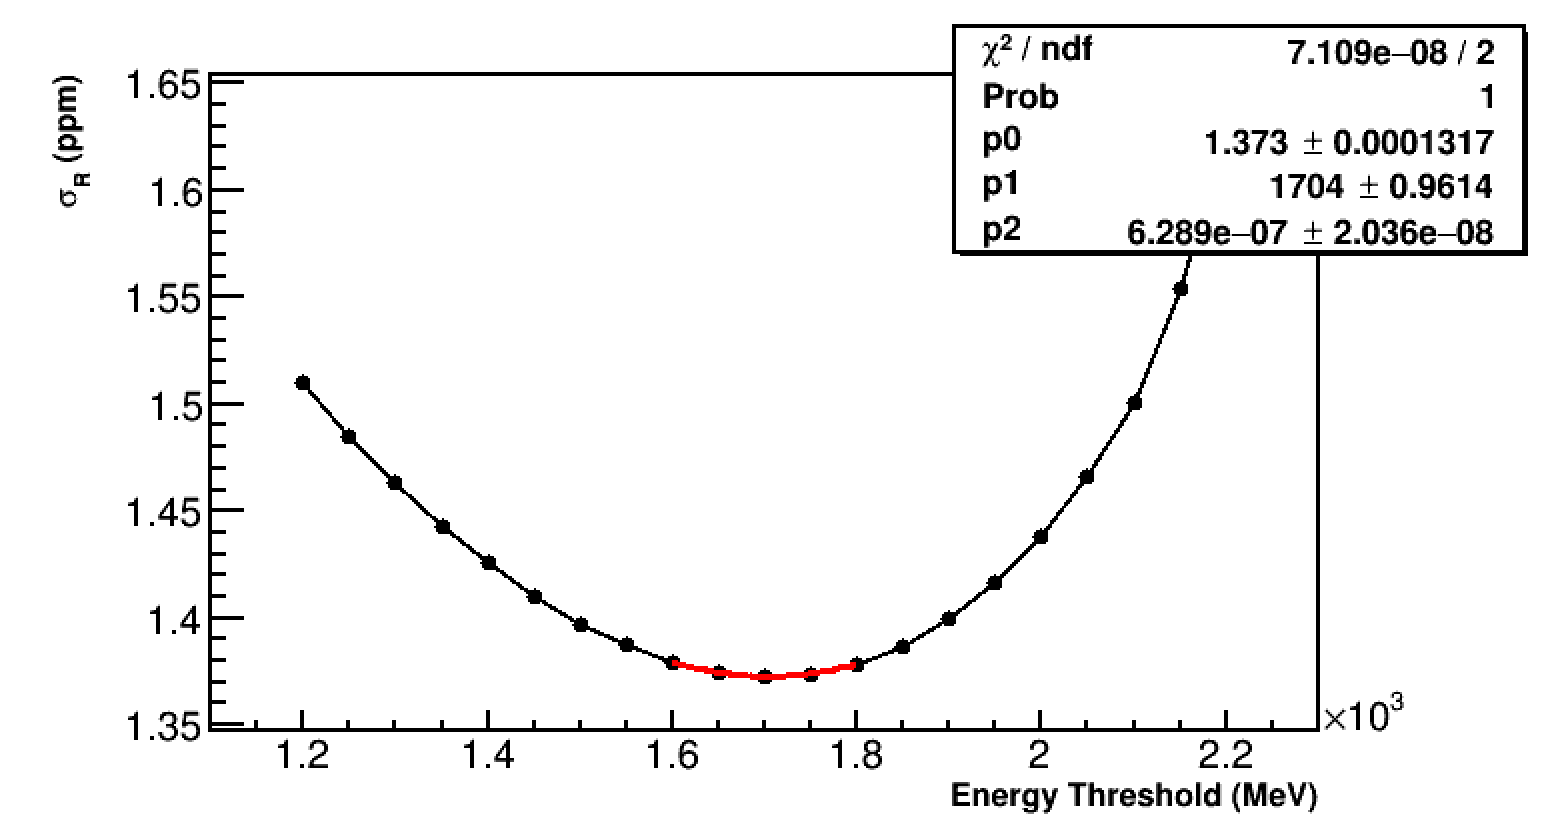
\includegraphics[width=\textwidth]{TemporaryEThresholdRatio}
            \caption{}
        \end{subfigure}% 
    \caption[Determination of optimal energy threshold]{The optimal energy threshold can be determined from the $NA^{2}$ quantity as described in \secref{section:WaIntro} from a five parameter fit to the data (left), or from the calculated error with the final fit function (right). \textbf{temporary energy threshold plots - replace - also not sure how to introduce R and ratio fit stuff here when I haven't talked about it yet}}
    \label{fig:OptimalEnergyThreshold}
    \end{figure}

% \begin{figure}[]
%     \centering
%     % \includegraphics[width=0.9\textwidth]{OptimalEnergyThreshold}
%     \rule{10cm}{10cm}
%     \caption[put caption here]{put a picture of the scanned optimal energy threshold here}
%     \label{fig:OptimalEnergyThreshold}
% \end{figure}


The optimal bin width for the time histograms was determined to be $\SI{149.2}{ns}$, the average of the cyclotron periods determined from a fast rotation analysis to the data \cite{fastrotationsomething}. As described in \secref{sub:beam_debunching}, this bin width combined with a time randomization on each cluster over a range of $\pm T_{c}/2 = \SI{149.2}{ns} / 2$ serves to eliminate the fast rotation signal in the data\footnote{Some analyzers randomize all times in a single fill by half the cyclotron period as opposed to each individual pulse.}. This randomization is done using \ROOT's \texttt{TRandom3} class. The default random seed for each histogram \ROOT file is the hash of the input file name using C++'s standard hash class. Histograms are defined with a time range of 0--\mus{699.8972} (the closest integer multiple of the bin width to \mus{700}), corresponding to 4691 bins. Clusters with times $<$ \mus{25} or $>$ \mus{660} are dropped, corresponding to 4256 bins containing data.




-include sam dataset names here or in the run 1 section?
-I should probably talk a little bit about the energy spectra as well
- need to mention how the spectra are split into different calorimeters
-should I show an energy spectra here without the pileup subtracted - I need to talk about the lost muon peak 


\subsection{Pileup subtraction}
\label{sub:pileupsubtraction}


As described in \secref{sec:Calorimeters}, there will be a certain amount of pileup in the detectors. Pileup again is the term for when multiple particles hit a calorimeter within the dead time of the detector such that they are registered as a single hit or cluster. The measured energy and time spectra for all observed clusters will include this pileup background. For the energy threshold time histogram, the number of counts will be wrong for cases where two below-threshold particles are registered as a single cluster above threshold, and where two above-energy threshold particles are registered as a single cluster. In the former, an extra count is added into the histogram, and in the latter a count is missed. The case where two lower energy positrons are registered as a single higher energy cluster will have a different \gmtwo phase than an actual single cluster at the same energy. This is because the lower energy positrons on average decay from muons which have travelled further around the ring, due to acceptance effects. These muons which have travelled further around the ring have spent more time in the magnetic field, and thus their spins have precessed more. See \figref{fig:PileupExample}. Clusters which originate from pileup events therefore have a different \gmtwo phase than non-pileup events. 


If pileup was a constant effect, then the phase of the time histogram would be shifted by some constant amount, and the extracted \wa frequency would be unaffected. However, the rate of pileup in the detectors changes over the time of a fill, as muons decay away. The rate of double pileup events in the detectors, where the word double indicates cases where two hits are registered as a single cluster, will go approximately as half the rate of single hit events\footnote{It is not exact when including the non-linear dead time of the detectors}, and similarly for triple and higher orders of the pileup effect. Because the rate of hits in the detectors oscillates at the \gmtwo frequency, pileup will increase and decrease accordingly leading to oscillations in the pileup time spectra at \wa and 2\wa. The lifetime of the overall pileup effect is approximately half the lifetime at which clusters are registered in the detectors, at \taumu, since double pileup is the dominant contribution. In order to to extract the correct \wa frequency, the pileup effect thus needs to be included in the fit function or subtracted out of the data. The former is challenging due to the non-linear nature of the dead time of the detectors, and would in the end include another phase in the argument of the cosine term in the fit function, thus worsening the statistical precision of the extracted \wa frequency. All analyzers thus construct an approximation of the pileup effect and subtract it from the data before fitting.


% -need to mention the \% level effect of pileup - ~1\% but where do you get that number...


\begin{figure}[]
    \centering
    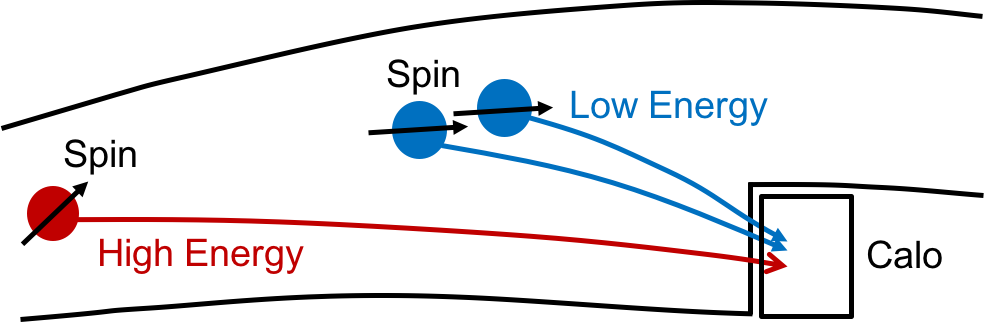
\includegraphics[width=0.5\textwidth]{PileupExample}
    \caption[Pileup example]{Pileup example, where two low energy positrons are registered as a single high energy positron. The black arrows indicate the (exaggerated) direction of the muon spins at the time of decay. Because of acceptance effects the lower energy decay positrons typically come from muons which have traveled further around the ring, and thus the muon spins have precessed more in the magnetic field, leading to a different measured \gmtwo phase for pileup events.}
    \label{fig:PileupExample}
\end{figure}


There are various methods to construct pileup spectra which are then subtracted off the main time and energy spectra. The method used in this analysis is called the `asymmetric shadow method', originally developed in E821 \cite{E821PileupShadow}. This method statistically constructs an approximation for the pileup from the data by assuming that the probability of observing a pileup pulse is the same as the probabilty that two pulses will be offset by some small amount of time, such as \ns{10}. The method works by looking in time windows after trigger pulses to see if a `shadow' pulse exists. If such a pulse exists, then a shadow doublet is created, see \figref{fig:ShadowPileupMethod}. The width of the time window, and the time offset from the trigger pulse to the window, are called the shadow dead time (SDT) and shadow gap time (SGT) respectively. The times and energies of the constructed pileup doublets are taken as
            \begin{gather}
                E_{\text{doublet}} = C \cdot (E_{1} + E_{2}), \label{eq:Edoublet} \\
                t_{\text{doublet}} = \frac{t_{1} \cdot E_{1} + (t_{2}-SGT) \cdot E_{2}}{E_{1} + E_{2}}, \label{eq:tdoublet}
            \end{gather}
where the energy of the doublet is the sum of the two singlet pulses $E_{1,2}$ times some calibration constant $C$, with a default value of 1, and the time of the doublet is the energy-weighted time of the two singlets $t_{1,2}$. The procedure for constructing the pileup spectra is as follows:
\begin{itemize}
    \item{Put each hit into a vector corresponding to a specific fill and a specific calorimeter}
    \item{Time order the hits}
    \item{Loop through the hits, for each hit look within a window of width SDT a time SGT later to see if a shadow pulse exists}
    \item{If a shadow pulse exists, construct a shadow doublet with energies and times as defined in Equations~\ref{eq:Edoublet} and \ref{eq:tdoublet}}
    \item{Randomize $t_{\text{doublet}}$ over the range $\pm T_{c}/2$ (to remove fast rotation as before, \secref{sub:beam_debunching})}
    \item{Per calorimeter, construct pileup energy and time spectra as $P = D - S$, where $D$ is the sum of doublets and $S$ is the sum of singlets used in the construction of the doublets, with the times of the singlets set as $t_{\text{doublet}}$; when constructing the pileup time spectra, only include those doublets and singlets above the energy threshold}
\end{itemize}
Thus pileup energy and time spectra are constructed for each calorimeter, which can then be subtracted off the calorimeter cluster energy and time histograms. When combining the data, the individual pileup histograms are simply added together before subtraction off the calorimeter sum histograms. 


In order to produce an estimate of the pileup spectra which best matches the data, an artifical dead time (ADT) is applied to the data before time randomization. This is done because the true dead time of the detectors depends on the energies and spatial separation of the incoming hits. While this is a small effect, by applying an artificial deadtime and matching the shadow window time, the pileup estimation is improved slightly. The construction of the artificial pileup is handled in the same way as the construction of the shadow pileup, with SGT set to \ns{0}. The constructed artificial doublets replace the singlets in the data. The value for the ADT and SDT is set at \ns{5}, the time threshold at which pileup is 100\% resolved. 

The value of the SGT is simply set to twice the SDT, in order to push the shadow window out to times well beyond the dead time of any pileup events, but not so far that an appreciable fraction of muons have decayed. The value of the doublet energy scaling factor C is set to 1, which is a fine approximation as the spatial separation in the reconstruction is turned off\footnote{With the spatial separation turned off, `pileup' events can occur in crystals that are easily separated by eye. While this increases the level of pileup seen in the data, the pileup approximation method also does not consider the spatial separation, and thus handles the level of pileup accordingly.}. The values for each pileup parameter is shown in \tabref{tab:histogramparameters}. See \secref{sub:pileuperror} for systematic studies on the effect on \wa due to these chosen parameters.



\begin{figure}[]
    \centering
    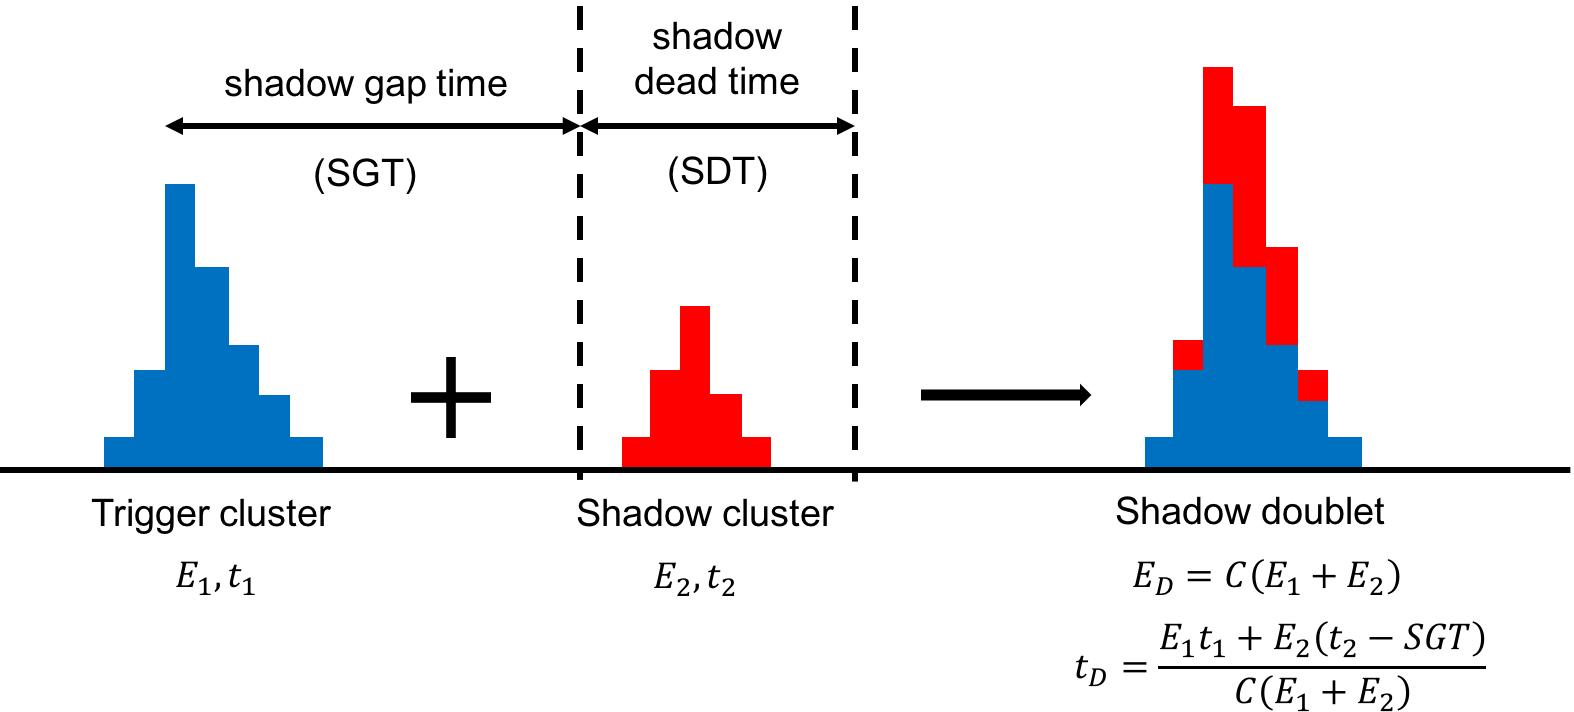
\includegraphics[width=\textwidth]{ShadowPileupMethod}
    \caption[Shadow pileup method]{}
    \label{fig:ShadowPileupMethod}
\end{figure}


The pileup energy spectra as compared to the cluster energy spectra is shown in \figref{fig:ClusterEnergiesVsPileupEnergies}. In general, the two lobes starting at approximately $\SI{3}{\GeV}$ and $\SI{6}{\GeV}$ consist of double and triple pileup events respectively\footnote{All orders of pileup fill out the whole energy range, but certain areas consist of mostly one or the other.}. It can be seen that the shadow method of pileup construction produces a pileup energy spectra which is a decent approximation of the cluster energies above the maximum energy that a single decay positron would have at $(\SI{3.094}{\GeV}) + \text{detector resolution}$, for cases of double and even triple pileup. The shape difference arises from two factors: First, the shadow method is only written to construct doublets, and does not consider cases of triple or higher orders of pileup. Second, the real pileup in the data contaminates the construction of the shadow pileup spectra, such that a shadow doublet can be constructed from real pileup pulses. While this alleviates the triplet problem slightly, it means that the doublet pileup spectrum is slightly wrong. The corrected energy spectra (cluster energies minus pileup energies), can be seen in \figref{fig:AddedEnergies}. The shape mismatch is even more apparent as the corrected energy spectrum is high for energies above the expected tail of the true energy distribution, and then goes negative before tailing off to zero. It has been determined that regardless of this shape mismatch, the systematic error on the extracted \wa frequency due to the pileup is within the target uncertainty for the level of statistics in the Run~1 dataset, \secref{sub:pileuperror}. This is in part due to the fact that it is the pileup time spectrum that is most important, as opposed to the pileup energy spectrum. The pileup time spectrum for those pileup pulses above energy threshold is shown in \figref{fig:PileupTimeSpectrum}. Finally, since the pileup is statistically constructed and then subtracted from the data, the errors on the final time histogram are no longer Gaussian. The proper calculation of the errors is detailed in \appref{app:PileupErrors}.


    \begin{figure}[]
        \centering
        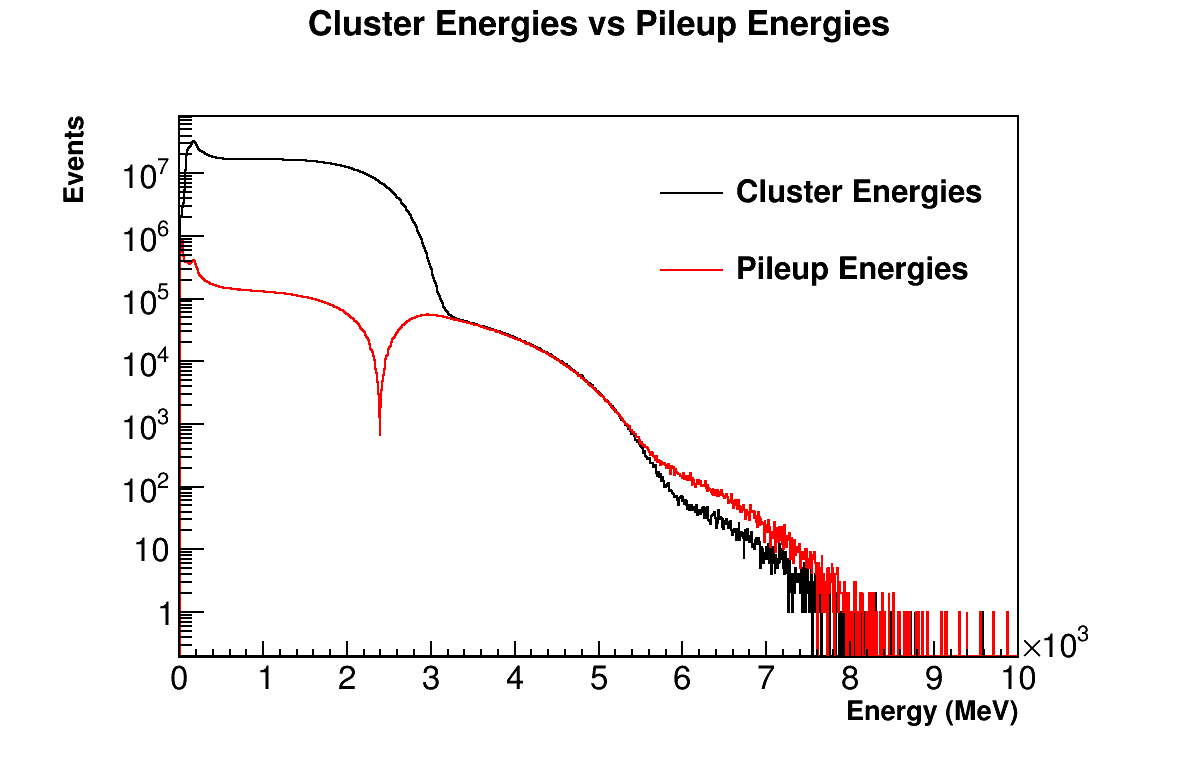
\includegraphics[width=\textwidth]{ClusterEnergiesVsPileupEnergies}
        \caption[Cluster energies vs pileup energies]{Cluster energies in black are plotted vs pileup energies in red, for all calorimeters added together, plotted on a log scale. At energies below about 2.4 GeV the pileup energy spectrum goes negative. In this plot the absolute value of the pileup energies is plotted, and a spike at about 2.4 GeV can be seen as a consequence of this. The shapes do not match perfectly for the constructed pileup spectra, which can be seen at high energies. It should be noted that for energies above $\SI{3.094}{\GeV}$ there is still a shape mis-match even though the red and black curves overlap due to the plotting scale.\textbf{update pictures with latest data, improved captions, and plotting styles}}    
        \label{fig:ClusterEnergiesVsPileupEnergies}
    \end{figure}


    \begin{figure}[]
    \centering
        \begin{subfigure}[]{0.8\textwidth}
            \centering
            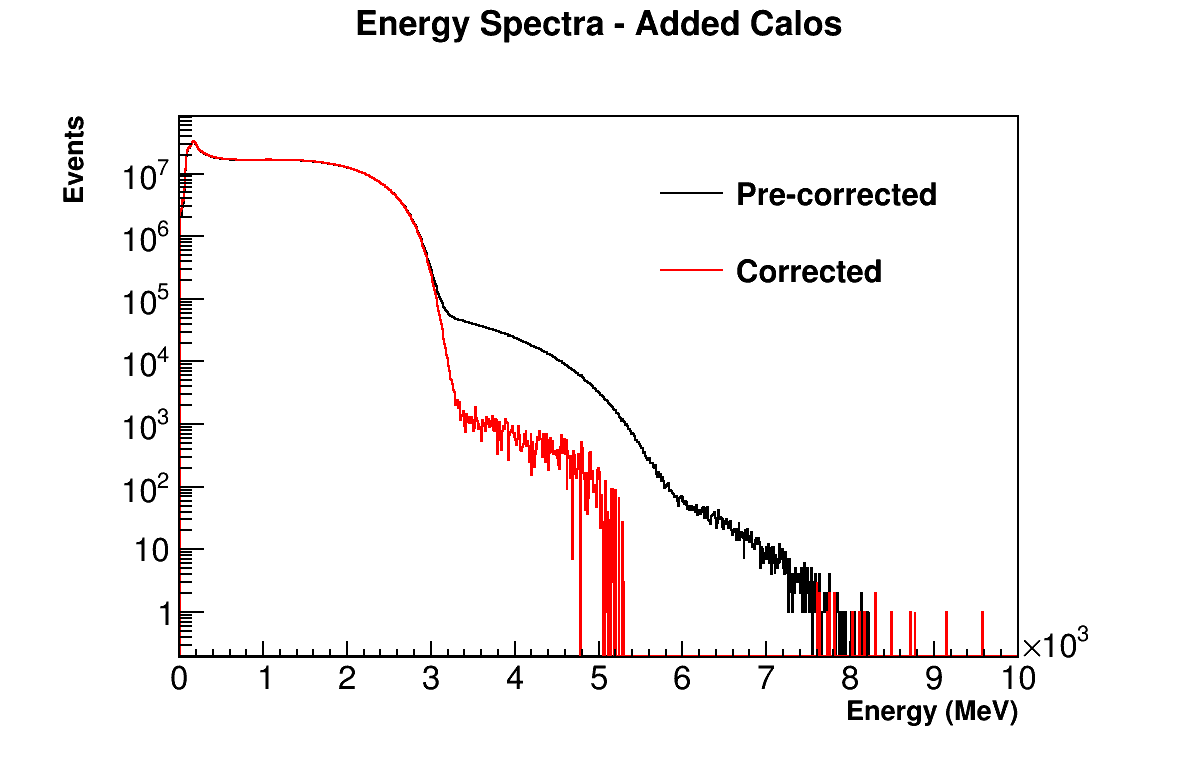
\includegraphics[width=\textwidth]{AddedEnergies}
            \caption{Log scale - the corrected energy spectrum goes negative around 5 GeV.}
        \end{subfigure}% %you need this % here to add spacing between subfigures
        \vspace{1cm}
        \begin{subfigure}[]{0.8\textwidth}
            \centering
            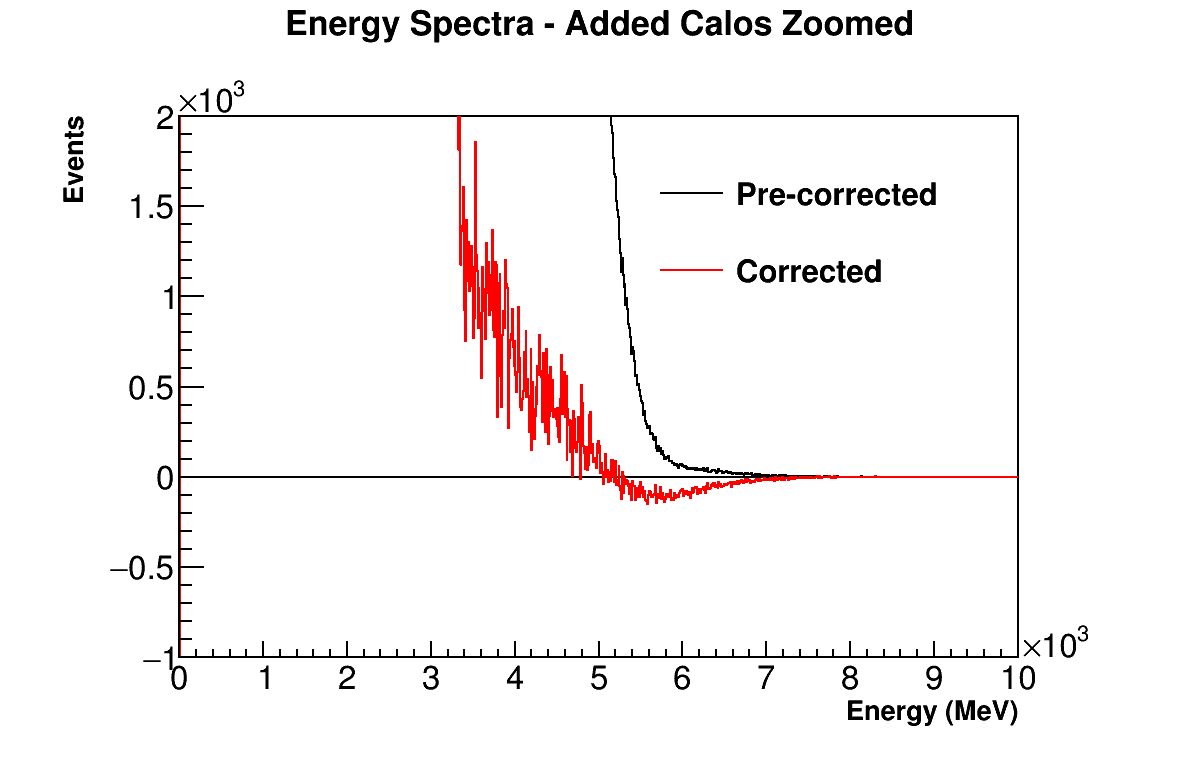
\includegraphics[width=\textwidth]{AddedEnergiesZoomed}
            \caption{Linear scale - zoomed in to show the shape.}
        \end{subfigure}
    \caption[Non-corrected and pileup corrected cluster energies]{Plots for the pre-corrected and corrected energy spectra are shown, all calorimeters added together. Because the triplets and contamination are not accounted for, the corrected energy spectrum does not lie exactly along zero above the energy response of the detectors.\textbf{update pictures with latest data, improved captions, and plotting styles}}
    \label{fig:AddedEnergies}
    \end{figure}


    \begin{figure}[]
        \centering
        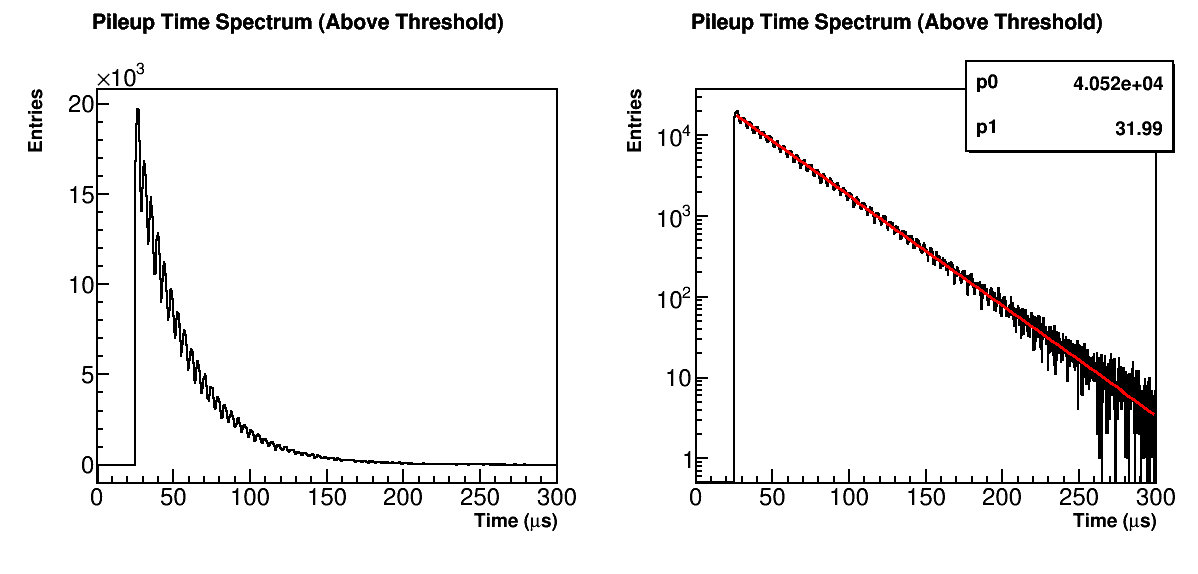
\includegraphics[width=\textwidth]{PileupTimeSpectrum}
        \caption[Pileup time spectrum above threshold]{Plotted is constructed pileup time spectrum on a linear (left) and log (right) scale. The histogram on the right is fit to a simple two parameter exponential to get an idea of the lifetime of the pileup, calculated here as $\SI{31.99}{\mu s}$, which is close to half of the muon lifetime at about $\SI{64.44}{\mu s}$.\textbf{update pictures with latest data, improved captions, and plotting styles}}
        \label{fig:PileupTimeSpectrum}
    \end{figure}





-should I show per calorimeter pileup energy and time spectra????



    % \begin{figure}[]
    %     \centering
    %     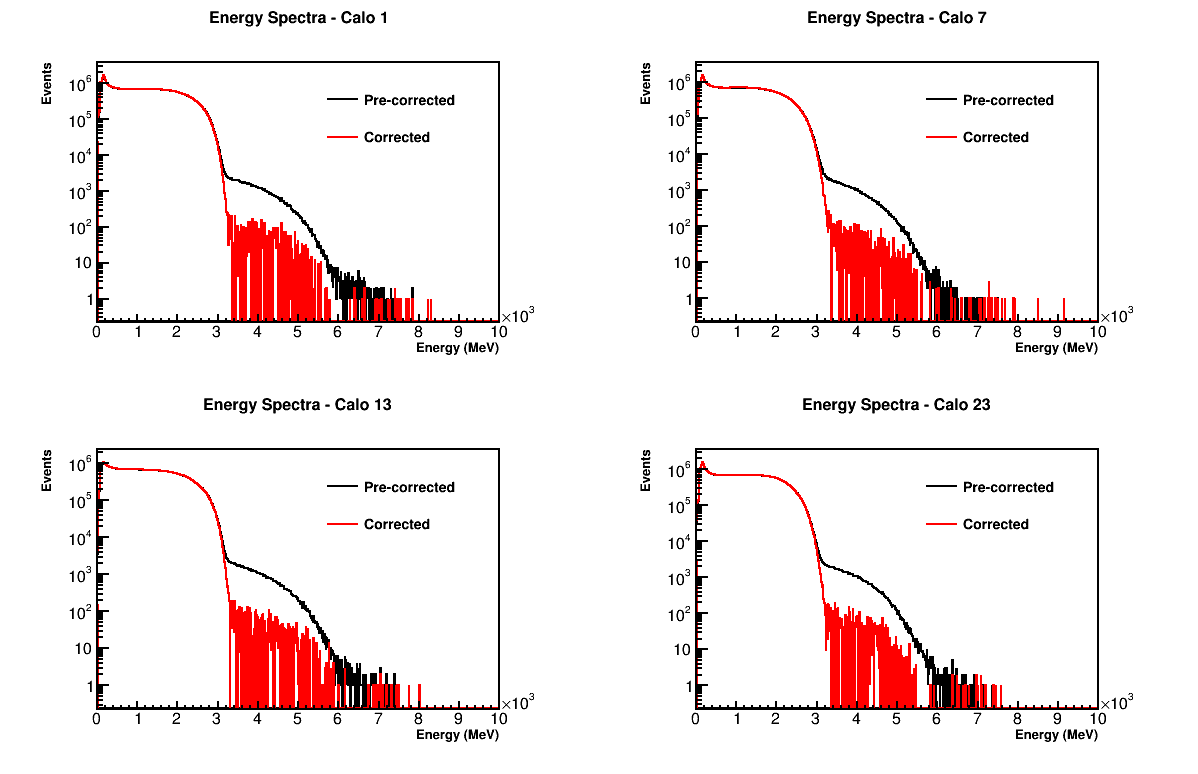
\includegraphics[width=.8\textwidth]{CaloEnergies}
    %     \caption[CaloEnergies]{Pre-corrected and corrected energy spectra for calorimeters 1, 7, 13, and 23 plotted on a log scale.}    
    %     \label{fig:CaloEnergies}
    % \end{figure}

    % \begin{figure}[]
    %     \centering
    %     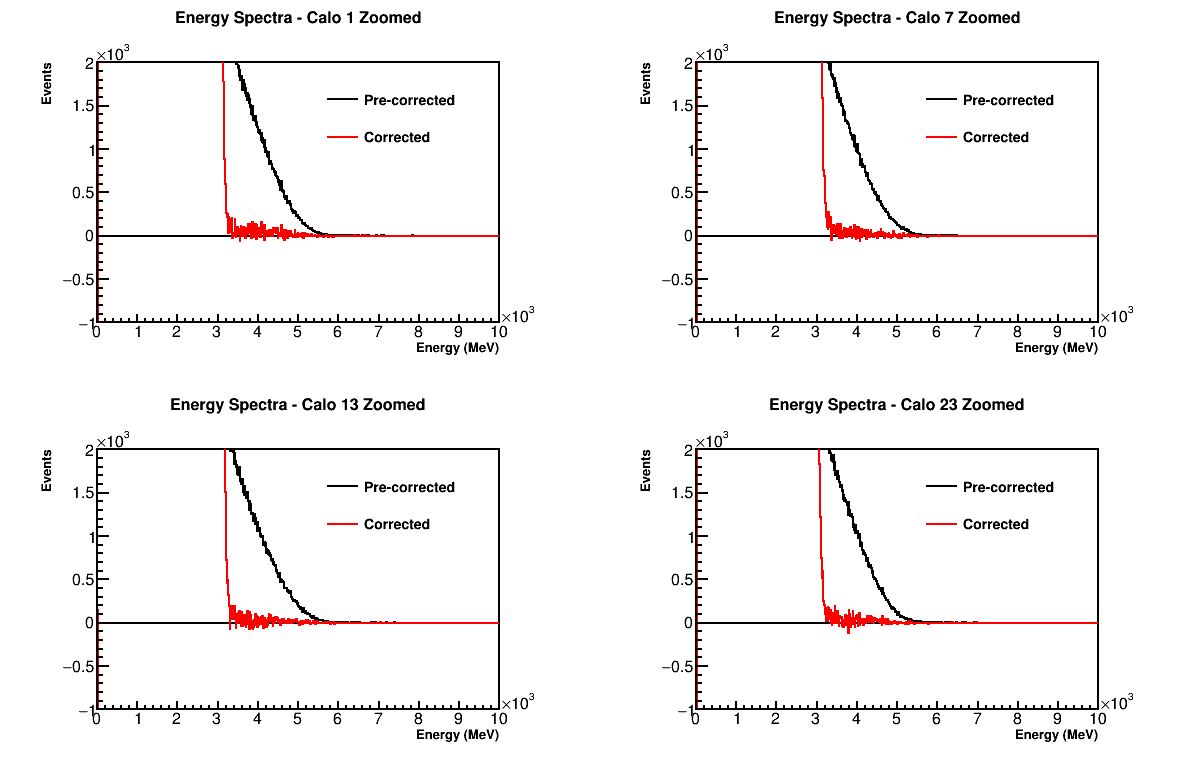
\includegraphics[width=.8\textwidth]{CaloEnergiesZoomed}
    %     \caption[CaloEnergiesZoomed]{Pre-corrected and corrected energy spectra for calorimeters 1, 7, 13, and 23 plotted on a linear scale and zoomed in.}    
    %     \label{fig:CaloEnergiesZoomed}
    % \end{figure}




% https://gm2-docdb.fnal.gov/cgi-bin/private/RetrieveFile?docid=13963&filename=PileupScaleShadowTesting.pdf&version=1
% https://gm2-docdb.fnal.gov/cgi-bin/private/RetrieveFile?docid=14394&filename=PileupFormEtc.pdf&version=2




\subsection{Ratio Method}


The method used in this analysis to extract \wa is called the ``Ratio Method.'' It is a technique that modifies the data in such a way that the exponential decay in the time histogram is removed, and slow effects are reduced. It was used successfully in the E821 experiment \cite{JKThesis,LDThesis,JPThesis}. A full derivation of the equations in the method is given in \appref{app:RatioDerivation}, here is given a short summary.

The method works by dividing the data into four separate datasets, one with the times of all clusters shifted up by half a \gmtwo period, $+$\Tatwo, one with times shifted down by half a \gmtwo period, $-$\Tatwo, and two left alone\. Assuming the data is described by the five parameter function \equref{eq:5parfunc} shown in \figref{fig:fiveparamfunc} (repeat it here?), and that the data is equally split into four, then the new four datasets are given as:
    \begin{equation}
    \begin{aligned}
        u_{+}(t) &= \frac{1}{4} N_{5}(t+T/2) \\
        u_{-}(t) &= \frac{1}{4} N_{5}(t-T/2) \\
        v_{1}(t) &= \frac{1}{4} N_{5}(t) \\
        v_{2}(t) &= \frac{1}{4} N_{5}(t)
    \end{aligned}
    \end{equation}
To be explicit here regarding the signs, the counts that are filled into the histogram described by $u_{+}$ have their times shifted as $t \rightarrow t - T/2$, which is what the function $N_{5}(t+T/2)$ describes, and vice versa for $u_{-}$footnote{When handling the pileup in the ratio method, the pileup time spectra are split into four datasets in the same way as the ratio method, where associated doublets and singlets are kept together, and the four datasets are individual subtracted off the four ratio datasets before forming the ratio.}. In order to time shift the data as such, \Ta needs to be known a priori to high precision. The value used is taken from the E821 result, and its value is taken as $1/f_{a}$, where $f_{a}$ is \SI{0.2290735}{MHz}:
        \begin{align}
            T_{a} \approx \SI{4.365411}{\mu s}
        \label{eq:Ta}
        \end{align}
This value for $f_{a}$ was determined by averaging column 2 of Table XV of the E821 Final Report \cite{E821FinalReport}, which consits of the $f_{a}$ results for the different run periods in that experiment. A systematic error on the choice of this parameter is calculated in \secref{sub:TimeShiftingParameters}.


The datasets are then combined as 
    \begin{equation}
    \begin{aligned}
        U(t) &= u_{+}(t) + u_{-}(t), \\
        V(t) &= v_{1}(t) + v_{2}(t),
    \label{eq:UandV}
    \end{aligned}
    \end{equation}
and shown in \figref{fig:UVfuncs}. It is immediately apparent that the $U(t)$ data are shifted 180\textdegree{} out of phase from the $V(t)$ data. The ratio is then defined as 
    \begin{align}
        R(t) &= \frac{V(t) - U(t)}{V(t) + U(t)}
    \label{eq:ratiointext}
    \end{align}
where the numerator and denominator are plotted in Figures~\ref{fig:rationumfunc} and \ref{fig:ratiodenomfunc} respectively. The numerator is seen to be an exponentially decaying cosine, while the denominator is a simple exponential, both of which can be seen as originating from the difference and sum of the $U(t)$ and $V(t)$ data respectively\footnote{The ratio can also be defined with $U(t) - V(t)$ in the numerator, but then the phase of the ratio spectrum will be shifted 180\textdegree{} from the original $N_{5}(t)$ spectrum.}. The resulting ratio spectrum can be seen in \figref{fig:ratiofunc}, where the exponential is seen to have been eliminated. The fit function is then reduced from 5 parameters down to 3:
    \begin{align}
        R(t) \approx A \cos(\omega_{a}t) - C,
    \label{eq:ratiowithC}
    \end{align}
where  
    \begin{align}
        C = \frac{1}{16} \Big(\frac{T}{\tau}\Big)^{2} \approx 2.87 * 10^{-4},
    \end{align}
and these functions have been determined from the time shifted five parameter function plugged into the $U(t)$ and $V(t)$ variables. In addition to the exponential being eliminated, any slow terms in the data get time shifted and then divided as well, such that such effects are reduced. In order to eliminate the constant $C$ at the end of \equref{eq:ratiowithC}, a different weighting scheme as opposed to equal weighting can be used as described in \refref{statisticspaper}:
    \begin{equation}
    \begin{aligned}
        u_{+}(t) &= \frac{e^{T/2\tau}}{2 + e^{T/2\tau} + e^{-T/2\tau}} N_{5}(t+T/2) \\
        u_{-}(t) &= \frac{e^{-T/2\tau}}{2 + e^{T/2\tau} + e^{-T/2\tau}} N_{5}(t-T/2) \\
        v_{1}(t) &= \frac{1}{2 + e^{T/2\tau} + e^{-T/2\tau}} N_{5}(t) \\
        v_{2}(t) &= \frac{1}{2 + e^{T/2\tau} + e^{-T/2\tau}} N_{5}(t).
    \label{eqn:fourHistsInText}
    \end{aligned}
    \end{equation}
where the factors out front are each close to $1/4$ and account for the amount of muon decay over \Tatwo, and $\tau = \tau_{\mu}$. In the latter case the muon lifetime must be known a priori, and it's value is taken as \mus{64.44}, determined from fits to the data. A systematic study regarding this parameter is described in \secref{sub:TimeShiftingParameters}. Both the values for \taumu and \Ta are given in \tabref{tab:histogramparameters}. The ratio spectrum is then almost exactly described by just the cosine term:
    \begin{align}
        R(t) \approx A \cos(\omega_{a}t),
    \end{align}



    \begin{figure}[]
    \centering
        \begin{subfigure}[t]{0.45\textwidth}
            \centering
            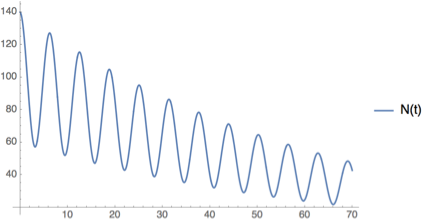
\includegraphics[width=\textwidth]{FiveParamFunc}
            \caption{The five parameter function defined in \equref{fig:fiveparamfunc}, which describes the incoming data at first order.}
        \label{fig:fiveparamfunc}
        \end{subfigure}%

        \vspace{2mm}
        \begin{subfigure}[t]{0.45\textwidth}
            \centering
            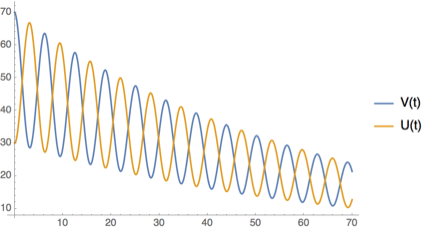
\includegraphics[width=\textwidth]{UVFuncs}
            \caption{The $U(t)$ and $V(t)$ functions which describe the time-shifted and unshifted datasets as described in the text.}
        \label{fig:UVfuncs}
        \end{subfigure}
        \hspace{5mm}
        \begin{subfigure}[t]{0.45\textwidth}
            \centering
            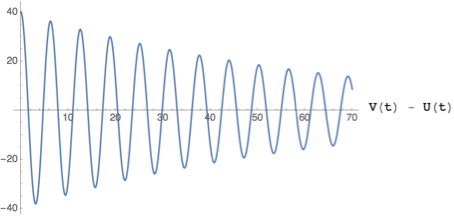
\includegraphics[width=\textwidth]{RatioNumFunc}
            \caption{The numerator function in the formed ratio, $V(t) - U(t)$. It is an exponentially decaying cosine.}
        \label{fig:rationumfunc}
        \end{subfigure}%
        \vspace{2mm}
        \begin{subfigure}[t]{0.45\textwidth}
            \centering
            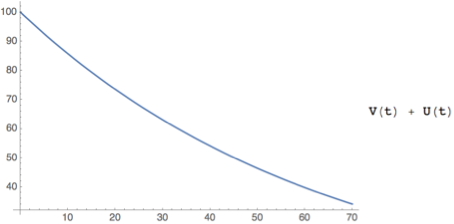
\includegraphics[width=\textwidth]{RatioDenomFunc}
            \caption{The denominator function in the formed ratio, $V(t) + U(t)$. It is an exponentially decaying curve.}
        \label{fig:ratiodenomfunc}
        \end{subfigure}
        \hspace{5mm}
        \begin{subfigure}[t]{0.45\textwidth}
            \centering
            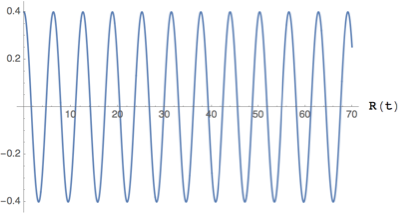
\includegraphics[width=\textwidth]{RatioFunc}
            \caption{The formed ratio function, describing the data after it has been handled as described in the text. To first order it is reduced to a simple cosine form.}
        \label{fig:ratiofunc}
        \end{subfigure}% 
    \caption[Ratio formation function]{Functions describing the formation of the ratio in the data. \textbf{should I just use the ones I make with the data or no?}}
    \label{fig:RatioFormationFunctions}
    \end{figure}



-read through 60h report and make sure I didn't miss anything



\section{Lost muons}
\label{sec:lostmuons}

-need to include delta t plot and energy deposition plot
-this should potentially be in the fitting section...


\cite{lostmuons}




\section{Fitting}
\label{sec:Fitting}


-should I include stuff about my tmethod fits? just basic fit results but no systematic studies and all that?
-a root macro is used to fit the data, and then to make plots


Fit is from \mus{30.2}--\mus{650}, corresponding to 4154 bins.


\begin{table}[]
\centering
\setlength\tabcolsep{10pt}
\renewcommand{\arraystretch}{1.2}
\begin{tabular*}{.8\linewidth}{@{\extracolsep{\fill}}lc}
  \hline
    \multicolumn{2}{c}{\textbf{Fit Procedure Parameters}} \\
  \hline\hline
    Parameter & Value \\
  \hline
    Fit start time & \mus{30.2} \\
    Fit end time & \mus{650} \\
  \hline 
\end{tabular*}
\caption[]{\textbf{fill this table out more once I've gone through the various parts}}
\label{tab:fitprocedureparameters}
\end{table}





\begin{gather}
    R(t) = \frac{2f(t) - f_{+}(t) - f_{-}(t)}{2f(t) + f_{+}(t) + f_{-}(t)} \\[6pt]
    f_{\pm}(t) = f(t \pm T_{a}/2) \\[6pt]
    f(t) = \Lambda(t) \cdot V(t) \cdot N_{cbo}(t) \cdot (1 + A_{cbo}(t) \cdot \cos(\omega_{a}t + \phi_{cbo}(t))) \\[6pt]
    N_{cbo}(t) = 1 + A_{cbo-N} \cdot e^{-t/\tau_{cbo}} \cdot \cos(\omega_{cbo}(t) \cdot t + \phi_{cbo-N}) \\[6pt]
    A_{cbo}(t) = A \cdot (1 + A_{cbo-A} \cdot e^{-t/\tau_{cbo}} \cdot \cos(\omega_{cbo}(t) \cdot t + \phi_{cbo-A})) \\[6pt]
    \phi_{cbo}(t) = \phi + A_{cbo-\phi} \cdot e^{-t/\tau_{cbo}} \cdot \cos(\omega_{cbo}(t) \cdot t + \phi_{cbo-\phi}) \\[6pt]
    \omega_{cbo}(t) = \omega_{cbo} \cdot (1 + \delta_{cbo}(t)) \text{, $\delta_{cbo}(t)$ fixed} \\[6pt]
    \Lambda(t) = 1 - \kappa_{loss} \int_{0}^{t} L(t')e^{(t'/\gamma\tau_{\mu})} dt' \\[6pt]
    V(t) = 1 + A_{VW} \cdot e^{-t/\tau_{VW}} \cos(\omega_{VW}t + \phi_{VW}) \\[6pt]
    \omega_{a} = 2 \pi \cdot \SI{0.2291}{MHz} \cdot (1 + R \times 10^{-6})
\end{gather}





\subsection{CBO terms}
\label{sub:cboterms}






\section{Systematic errors}
\label{sec:Systematic Errors}



\begin{table}[]
\centering
\setlength\tabcolsep{10pt}
\renewcommand{\arraystretch}{1.2}
\begin{tabular*}{.8\linewidth}{@{\extracolsep{\fill}}lc}
  \hline
    \multicolumn{2}{c}{\textbf{\wa Measurement Uncertainties}} \\
  \hline\hline
    Source of uncertainty & E989 Goal (ppb) \\
  \hline
    Gain changes & 20 \\
    Pileup & 40 \\
    Lost muons & 20 \\
    CBO & 30 \\
    E field and pitch corrections & 30 \\
  \hline
    Quadrature sum & 70 \\
  \hline 
\end{tabular*}
\caption[Uncertainties in the precession frequency measurement]{Systematic errors in the precession frequency measurement. \textbf{fill this table out more once I've gone through the various parts}}
\label{tab:wauncertainties}
\end{table}




\subsection{Gain}
\label{sub:gainerror}


-talk about the equations here - slight reference to either detector section or reconstruction section in this chapter



\subsection{Pileup}
\label{sub:pileuperror}


For errors relating to the choice of SDT and SGT - the idea is this: Show the plots which show how the choices of SDT and SGT don't matter as long as the automatic pileup scaling is applied (shapes are the same) - this implies that the error due to these guys is contained within the pileup multiplier error, and can thus be ignored in favor of the latter - point back to pileup section when talking about this - I can also potentially if I have time do scans on these parameters and look at the effect on R

% https://gm2-docdb.fnal.gov/cgi-bin/private/RetrieveFile?docid=13963&filename=PileupScaleShadowTesting.pdf&version=1
% https://gm2-docdb.fnal.gov/cgi-bin/private/RetrieveFile?docid=14394&filename=PileupFormEtc.pdf&version=2


-pileup multiplier - amplitude
-pileup time shift - phase
-pileup energy scaling - phase



\subsection{gm2 period guess and muon lifetime}
\label{sub:TimeShiftingParameters}


\cleardoublepage
